% \author wo
\documentclass[12pt, UTF8, AutoFakeBold]{ctexart}
\usepackage{xeCJK}
\usepackage{times}
\usepackage{pdfpages}
\usepackage{geometry}
\usepackage{enumerate}

\geometry{a4paper, left=2.4cm, top=2.4cm, right=2.4cm, bottom=2.4cm}

\setCJKmainfont{SimSun}
\setmainfont{Times New Roman}


\title{基于深度学习的小麦病害分类模型特征分析}
\date{}
\author{马群}
% \date{2019年2月22日}

% 英文摘要
\newcommand{\enabstractname}{Abstract}
\newenvironment{enabstract}{%
    \par\small
    \noindent\mbox{}\hfill{\bfseries \enabstractname}\hfill\mbox{}\par
    \vskip 2.5ex}{\par\vskip 2.5ex}

\begin{document}

% 定义字体
\newcommand{\song}{\CJKfamily{song}}    % 宋体
\newcommand{\fs}{\CJKfamily{fs}}        % 仿宋体
\newcommand{\kai}{\CJKfamily{kai}}      % 楷体
\newcommand{\hei}{\CJKfamily{hei}}      % 黑体
\newcommand{\li}{\CJKfamily{li}}        % 隶书

\newcommand{\yihao}{\fontsize{26pt}{36pt}\selectfont}         % 一号, 1.4 倍行距
\newcommand{\erhao}{\fontsize{22pt}{28pt}\selectfont}         % 二号, 1.25倍行距
\newcommand{\xiaoer}{\fontsize{18pt}{18pt}\selectfont}        % 小二, 单倍行距
\newcommand{\sanhao}{\fontsize{16pt}{24pt}\selectfont}        % 三号, 1.5倍行距
\newcommand{\xiaosan}{\fontsize{15pt}{22pt}\selectfont}       % 小三, 1.5倍行距
\newcommand{\sihao}{\fontsize{14pt}{21pt}\selectfont}         % 四号, 1.5 倍行距
\newcommand{\banxiaosi}{\fontsize{13pt}{19.5pt}\selectfont}   % 半小四, 1.5倍行距
\newcommand{\xiaosi}{\fontsize{12pt}{18pt}\selectfont}        % 小四, 1.5倍行距
\newcommand{\dawu}{\fontsize{11pt}{11pt}\selectfont}       % 大五号, 单倍行距
\newcommand{\wuhao}{\fontsize{10.5pt}{15.75pt}\selectfont}    % 五号, 单倍行距

% \begin{center}
    
\includegraphics[height=1.53cm,width=7.00cm,bb=0 0 887 191]{resource/nefu_pic.png}
\end{center}
  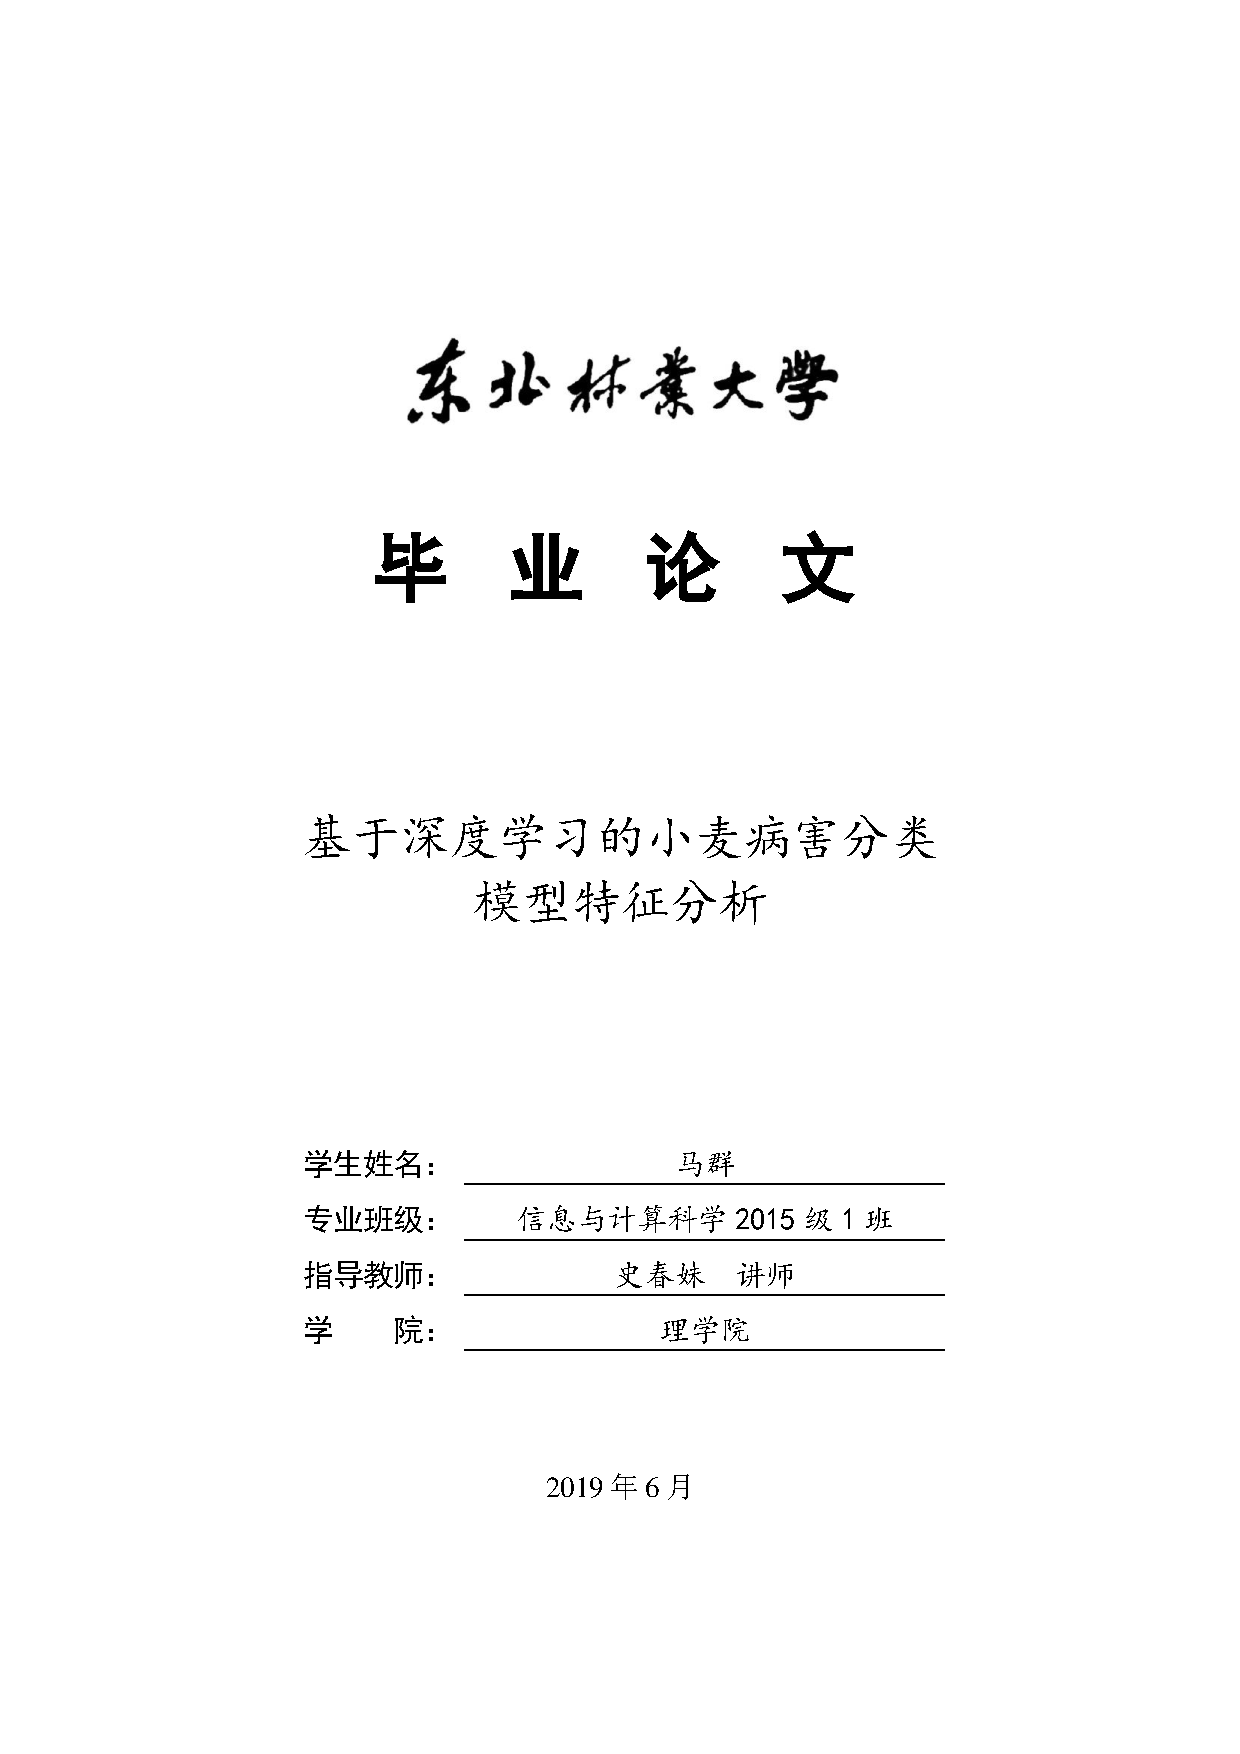
\includepdf{cover/cover.pdf}

  \maketitle
  \begin{abstract}
    为了实时监控小麦病害情况并及时采取防治措施,找出一种适合分类处理小麦常见病害的神经网络模型。
    本文首先以小麦病害图片资料为基础,经过挑选、裁剪后对图像进行序列化操作形成数据集,
    然后通过构建的多个深度神经网络模型进行学习,并利用随机梯度下降法进行学习过程控制。
    然后在此基础上改进表现较差的神经网络模型,在两个维度上形成对比,以此寻找最适合处理
    小麦病害分类问题的深度神经网络模型。实验结果表明,在参与实验的多个神经网络结构中,
    以卷积神经网络(convolutional neural networks,CNN)表现最为出众,
    整体识别准确率达99\%,(交叉)验证准确率在(validation accuracy)75\%左右。
    这表明卷积神经网络在小麦常见病害的识别中是有效且可行的,为小麦病害实时分析提供了有效分析手段。

    \leftline{\textbf{关键字 } \@ 小麦病害;卷积神经网络;卷积深度置信网络}
\end{abstract}
\newpage

\begin{center}
    \fontsize{18pt}{18pt}\textbf{Feature analysis of wheat disease classification model based on deep learning}
\end{center}
\begin{enabstract}
    This is the abstract in English.    This is the abstract in English.    This is the abstract in English.    This is the abstract in English.    This is the abstract in English.

    \leftline{\textbf{Keywords } \@ Wheat disease; Convolutional Neural Network; Convolutional deep belief networks}
\end{enabstract}
\newpage

  \tableofcontents % 目录
  \newpage

  \section{\hei\xiaoer\textbf{前言}}
  \setcounter{page}{1} % 设置页码起始
\subsection{\textbf{研究背景及意义}}
	小麦是我国三大粮食作物之一,其种植区域主要分布在长江以北的大部分地区,
	种植面积位居第二,仅次于水稻。病害是影响小麦等
	农作物产量和质量的首要问题。全世界范围内小麦病害大约有200多种,每年造成的产量
	损失约为15\%\textasciitilde20\%\upcite{CGRIS}。在我国危害较严重的有三十多种,其中以白粉病(Wheat powdery mildew)、
	锈病(Puccinia striiformis West,包括条锈、杆锈、叶锈)、叶枯病(Wheat leaf blotch)、
	赤霉病等在我国主要小麦产地分布较广,为害较为严重。

	传统形式的小麦病虫害是依靠经验识别、人工喷施农药进行防治的。在大面积的小麦种植模式下,人工防
	治不仅需要大量的人力物力,而且在喷施农药的过程中极为不安全。更进一步地讲,即使是在技术人员的
	帮助下进行病害防治,也不能做到实时监控小麦病害情况、及时实施防治工作。因此如何做到实时监控并
	报告小麦病害情况成为了现代农业生产中的重要目标。

	自1980年机器学习被称为一个独立的方向开始,经过一代又一代人的努力,诞生出了大量经典的分类算法。
	其中以朴素贝叶斯(Naive Bayes, NB)、K-均值聚类(k-means clustering)、逻辑回归(Logistic Regression, LR)、
	决策树(Decision Tree, DT)、支持向量机(Support Vector Machine, SVM)
	等浅层机器学习模型最为常用,
	它们的出现为小麦病害的自动识别提供了有力的理论支持。但是这些经典分类算法的图像特征提取策略是基
	于先验知识制定的,效率不高且不适合应用在大规模特征提取方面\upcite{article1}。 近年来,由AlphaGo
	带来的人工智能热潮使得深度学习一词出现在公共视野里。 深度学习是机器学习领域中一种以人工神经网络
	为架构,通过数据进行表征学习的算法。

	如此一来,将现代的深度学习技术与传统图像处理相结合的方式成为了农作物病害识别的新手段。深度学习在
	图像处理领域的优势不仅仅在于能够准确地提取特征,还在于它通过处理大量图像数据时能不断地自我学习并
	取得更高的准确率。

	在以深度学习为主要手段的图像处理过程中,卷积神经网络模型对图像的处理由很高的优势,故本文研究的内
	容会以卷积神经网络为基础,通过建立不同结构的神经网络模型并加以比较,找出最适合小麦病害识别的深度
	网络模型。
 
  \subsection{\hei\xiaosan\textbf{农作物病害识别的国内外研究现状}}
  \subsubsection{\hei\sihao\textbf{国内研究现状}}
    国内在农作物病害识别方面的研究起步较晚,多数是在国外相关研究启发下开始的。
    近年来机器学习领域的研究呈现井喷式发展,随之带动了农作物病害识别的研究,
    并取得了许多卓有成效的识别技术。
    2009年,王守志等实现了基于核K-均值聚类方法的玉米叶部病害识别,实验涉及的4
    种玉米病害识别准确率达82.5\% \upcite{王守志2009基于核};
    2011年,陈丽等提出了一种基于图像处理技术和概率神经网络技术的玉米叶部病害识
    别方法,利用遗传算法优化选择出4个分类能力强的分类特征,由概率网络(PNN)分
    类器识别病害,平均准确率为90.4\%,高于BP神经网络\upcite{陈丽2011概率神经网络在玉米叶部病害识别中的应用};
    % 张建华等提出了一种基于粗糙集和BP神经网络的棉花病害识别方法,
    % 该方法能准确识别4种棉花病害,平均识别准确率达到92.72\% \upcite{张建华2012基于粗糙集和};
    2012年,王树文等利用基本图像处理方法对黄瓜叶部病害图像进行处理,综合运用二次分割、
    形态学滤波得到病斑区域。提取三种特征并采用BP算法训练多层前向神经网络对
    黄瓜病害进行分类,该系统的平均识别准确度为95.31\% \upcite{王树文2012基于图像处理技术的黄瓜叶片病害识别诊断系统研究};
    2013年,张飞云等利用量子神经网络进行玉米病害分类识别,对玉米灰斑病、玉米普
    通锈病和玉米小斑病的识别准确率达92.5\%、97.5\%和92.5\%,高于误差反向传播
    神经网络法的识别率(分别为90.0\%、90.0\%和92.5\%),可用于玉米叶部病害识
    别\upcite{张飞云2013基于量子神经网络和组合特征参数的玉米叶部病害识别}。
    % 2014年,余秀丽等设计并实现了一种基于SVM(Support Vector Machine,支持向量机)
    % 的小麦叶部常见病害识别方法。随机试验结果表明,利用所提取的特征可以有效地实
    % 现小麦叶部常见病害的识别,基于形状特征综合识别率可达99.33\%,利用支持向量
    % 机算法进行小麦病害叶片识别是有效的、可行的\upcite{余秀丽2014基于};
    % 2018年,张航等提出了一种基于卷积神经网络的小麦病害识别方法,利用随机梯度
    % 下降法对一个具有五层结构的网络模型行学习过程控制,其综合识别率可达99\% 
    % \upcite{张航2018一种基于卷积神经网络的小麦病害识别方法}。

  \subsubsection{\hei\sihao\textbf{国外研究现状}}
    国外关于农作物病害识别的研究起步较早,在上世纪九十年代已有多种识别方法被提出。
    在早期的处理方法大多是对病害图像进行前期处理,包括图像分割、滤波、简单分类等
    技术,或是辅助以人工分析,然后再结合农作物病理学知识对处理后的数据进行分类识别。
    1997年,Tucker与Chakraborty提供了一种专用软件,可以检测向日葵和燕麦叶片上的病
    变,提供病变数量和类型以及病害严重程度的数据,但是该软件的分类准确率达不到预想
    程度 \upcite{tucker1997quantitative};
    1999年,Sasaki等使用光谱反射特性和滤光片图像构建了一个植物病害自动诊断系统,
    发现500、600和650mm的滤光镜图像比其他滤光镜图像更适合于识别,在创建鉴别参数对
    健康叶片和患病叶片进行分类后,达到了5\%或更小的误差率\upcite{sasaki1999automatic}。

    由于图像处理技术的限制,早期的农作物病害识别技术并不能满足人们的要求。近年来,
    随着图像处理和人工智能的发展,机器学习应用到农作物病害识别领域的例子越来越多。
    2008年,Phadikar和Sil等介绍了一种基于水稻植株感染图像的水稻病害检测系统,该
    系统使用图像生长、分割技术处理感染部分,然后使用SOM神经网络将四种叶子的感染部
    分进行分类处理,实验结果令人满意\upcite{phadikar2008rice};
    2014年,Mathura与Uttar Pradesh介绍了一种基于邻近像素点像素强度的改进和差直方
    图,与梯度滤波器相配合使用可以对苹果病害的检测达到99\%的准确率 \upcite{dubey2014fruit};
    2016年,Sladojevic等实现了最新一代的卷积神经网络(CNN),该模型能够识别健康
    叶片中的13种不同类型的植物病害,实验结果的平均精确度达到了96.3\% \upcite{sladojevic2016deep};
    2017年,Fuentes和Yoon等提出了一种深度学习方法来检测番茄病害,该方法含有三种
    神经元架构:基于区域的快速卷积网络(Faster R-CNN)、基于区域的全卷积网络
    (R-FCN)和单发多核检测器(SSD),实验结果表明,该系统能有效识别九种不同类型
    的病虫害\upcite{fuentes2017robust}。

\subsection{\hei\xiaosan\textbf{深度学习与神经网络的发展}}
  深度学习是机器学习领域中一种以人工神经网络为架构,根据数据进行表征学习的算法。
  它的前身是人工神经网络,基本特点是模仿人脑神经元处理和传递信息的方式,本质是解决贡献度的分配问题。

  对深度学习的研究最早可以追溯到1943年,数学家皮兹(W.Pitts)和神经科学家麦卡洛克
  (W.S.McCulloch)建立了一个基于神经网络和数学的模型,称为MCP模型。该模型是按照人脑神经元的结构和工作
  原理构造出来的一个抽象的、简化了的模型,也被人们称为“模拟大脑”\upcite{mcculloch1990logical}。
  1958年,计算机科学家罗森布拉特(Rosenblatt)提出了感知器(Perceptrons),
  这是一个由两层神经元组成的神经网络。这也是第一次将MCP模型用于机器学习分类。
  “感知器”算法使用MCP模型对输入的多个维度数据分为两类,且能够在训练过程中中自
  动优化并更新权值。1962年,Novikoff定理证明该方法具有收敛性,理论与实践效果引起第一次神经网络热潮。

  神经网络之父Geoffery Hinton于1986年发明了适用于多层感知器(MLP)的BP(Backpropagation)
  算法,该方法采用Sigmoid进行非线性映射,有效解决了非线性分类和学习的问题。
  Sigmoid函数的输出在(0,1)内,单调连续且易于求导,非常适合用作输出层。
  但是它也有软饱和性的缺点,一旦落入饱和区,$f'(x)$就会变得接近于0,很容易产生梯度消失。
  90年代中期,支持向量机(Support Vector Machine,SVM)算法诞生,随之各种浅层机器学习
  模型被提出。支持向量机又名支持向量网络,是在分类与回归分析中分析数据的监督式学习模型与相关的学习算法\upcite{cortes1995support}
  支持向量机与其他浅层机器学习算法的提出再次使深度学习的发展受到阻碍。
  % 2006年Geoffrey Hinton和Ruslan Salakhutdinov提出了深层网训练中梯度消失的解决方案:
  % 无监督预训练下对权值进行初始化,有监督训练权值微调\upcite{hinton2006reducing}。2011年,ReLU
  % 激活函数被提出,该激活函数能够有效的抑制梯度消失问题。

  % 2011年,微软首次将深度学习应用在语音识别领域,取得了重大突破。微软研究院和Google的语音识别
  % 研究人员先后采用卷积神经网络使语音识别错误率降低20%\textasciitilde30%,是语音识别领域十多年来的突破性进展。
  Hinton所带领的课题组为了测试深度学习模型的能力,于2012年使用首次使用CNN网络AlexNet参加ImageNet
  图像识别比赛,在ImageNet评测上将错误率从26\%降低到15\%,在第二名(SVM方法)面前以压倒性的优势夺得
  冠军。
  % CNN也正是由于该比赛吸引到了众多研究者的注意。AlexNet的创新点在于:

  % \begin{enumerate}[(1)]
  %   \dawu\item 采用ReLU激活函数,大幅增加收敛速度并且从根本上解决了梯度消失的问题。
  %   \dawu\item 抛弃了“预训练+微调”的方法,完全采用有监督训练方式。同时也影响了深度学习主流学习方法
  %     使其因此变为了纯粹的有监督学习。
  %   \dawu\item 扩展了LeNet5的结构,添加Dropout层减小过拟合,LRN(局部影响归一化)层增强泛化能力并减小过拟合。
  %   \dawu\item 第一次使用GPU加速模型计算。
  % \end{enumerate}

  % 2016年3月,由谷歌(Google)公司开发的AlphaGo(基于深度学习算法)与围棋世界冠军、职业
  % 九段棋手李世石进行围棋大战,以4比1的总比分获胜;2016年末至2017年初,该程序在中国棋类网站上
  % 注册名为“大师”(Master)的帐号并与中日韩数十位围棋高手进行快棋对决,连赢60局,无一败绩;2017年5月,
  % 在乌镇围棋峰会上,AlphaGo与世界排名第一的围棋冠军柯洁对战,以3比0的最终比分获胜。围棋界公认
  % 阿尔法围棋的能力已经超过人类职业围棋顶尖水平。

  深度学习虽然已经成为众多科研领域的热门研究内容,但是目前还处于发展阶段,不管是理论方面还是实践
  方面都还有许多问题待解决,不过由于我们处在了一个“大数据”时代,以及计算机处理能力的大大提升,
  新理论的验证周期会大大缩短,人工智能的发展必然会很大程度地改变这个世界。

  \subsection{\hei\xiaosan\textbf{论文结构和研究内容}}
  \subsubsection{\hei\sihao\textbf{主要研究内容}}
    本文以提高卷积网络在小麦病害图像识别的准确率为目标,提出了具有12层结构的卷积网络。
    针对前期实验的不足之处对网络结构加以更改,在得到了训练过程中表现良好的网络模型的模型之后,
    将其与经典卷积网络模型LeNet-5、AlexNet的实验结果进行比较,分析本文模型的长处与不足,验证
    该模型在小麦病害图像识别中的有效性。
    

  \subsubsection{\hei\sihao\textbf{论文结构}}
    第一章是引言,首先介绍了小麦病害图像识别的研究背景和意义,
    然后综述了深度学习与神经网络的发展历史及研究现状,
    最后介绍了本文的主要研究内容和章节安排。

    第二章主要介绍了卷积的基础理论知识,然后简单介绍了卷积神经网络的发展及其特点和主要结构层次。

    第三章搭建了一个结构上较新颖的卷积神经网络模型,并针对小麦病害识别加以修改,
    使其尽量符合预期要求。接下来主要介绍了实验内容,首先是数据源的获取和处理,然后是不同模型
    在相同数据源下的训练过程。

    第四章是针对该实验结果的分析以及对不同模型的结果加以对比,说明本文新模型的优势。
    然后对数据集的质量进行了解释,以及数据集对训练结果的影响。最后是对本文的总结分析。

  \newpage

  \section{\hei\xiaoer\textbf{卷积神经网络}}
    \subsection{卷积}
  卷积(Convolution)是分析数学中的一种积分变换的方法,是其中一个函数反转并平移后与另一个
  函数乘积的积分。设$f$与$g$是$\mathbf{R_1}$上的两个可积函数,做积分后的新函数就成为函数
  $f$与$g$的卷积:
  \[f*g=\int_{\tau \in A}f(\tau)g(t-\tau) d\tau\]

  卷积也经常应用在图像处理中,因为图像是一个二维结构,所以适合用二维卷积对图像做特征提取等操作。
  给定一个图像$\mathbf{I}\in \mathbb{R}^{M\times N}$,
  和滤波器 $\mathbf{K}\in \mathbb{R}^{M\times N}$,
  一般$m<<M$,$n<<N$,其卷积为:
  % \[y_{ij}=\sum_{u=1}^m \sum_{v=1}^n w_{uv}\cdot x_{i-u+1,j-v+1}\]
  \begin{equation}
    S(i,j)=(I*K)(i,j)=\sum_m \sum_n I(m,n)K(i-m,j-n)
    \label{Formula.Second.1}
  \end{equation}
  下式为二维卷积示例:
  \begin{equation}
    {\begin{pmatrix}
    2& 0& 1& 1& 1 \\
    -1& 0& -3& 0& 1\\
    2& 1& 1& -1& 0 \\
    0& -1& 1& 2& 1 \\
    1& 2& 1& 1& 1
    \end{pmatrix}} 
    \otimes 
    {\begin{pmatrix}
      1& 0& 0\\
      0& 0& 0\\
      0& 0& -1
    \end{pmatrix}}
    =
    {\begin{pmatrix}
      -1& 1& -1\\
      2& 2& 4\\
      -1& 0& 0\\
    \end{pmatrix}}
    \label{Formula.Second.2}
  \end{equation}

  卷积是可交换的,我们可以等价地把(2-1)式写作:
  \begin{equation}
    (\ref{Formula.Second.1}) \Leftrightarrow S(i,j)=(K*I)(i,j)=\sum_m \sum_n I(i-m,j-n)K(m,n)
    \label{Formula.Second.3}
  \end{equation}
  (\ref{Formula.Second.3})式也被称为I和K的互相关(Cross-Correlation),它是一个衡量两个序列相关性的函数。通过(\ref{Formula.Second.1})、
  (\ref{Formula.Second.3})两式对比可知,卷积和互相关的区别仅仅在于卷积核是否进行了翻转(Flip)。许多机器学习库中实现的
  “卷积运算”其实是互相关函数,之所以称之为卷积运算,这是因为卷积核的特征提取能力与其是否翻转无关。在训练
  过程中,学习算法会在核合适的位置自动更新为恰当的值,所以一个基于互相关学习算法所学习到的核,是使用卷
  积运算所学到的核的翻转。

  数字图像是二维图像用有限数字数字像素的表示\cite{wiki:xxx},对数字图像做卷积操作其实是在图像上滑动一个卷积核(即滤波器),
  将图像点上的像素值与卷积核对应位置的值相乘,然后将相乘后所有的值相加,作为特征图像上对应位置的像素值。
  图\ref{Figure.Second.1}展示了(\ref{Formula.Second.2})中反转前后的卷积核在小麦锈病图像中特征提取效果的对比图。
  \begin{figure}[H]
    \centering %图片全局居中
    \subfigure[原图]{
      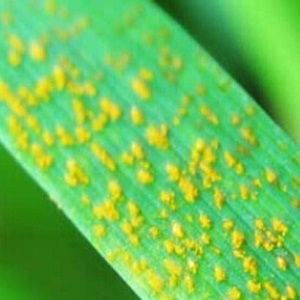
\includegraphics[width=0.2\textwidth]{resource/2-原图.jpg}
    }
    \subfigure[互相关]{
      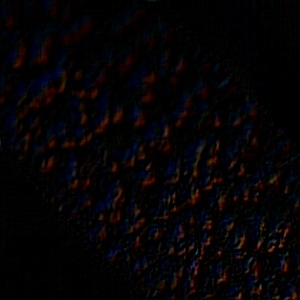
\includegraphics[width=0.2\textwidth]{resource/2-互相关.jpg}
    }
    \subfigure[卷积]{
      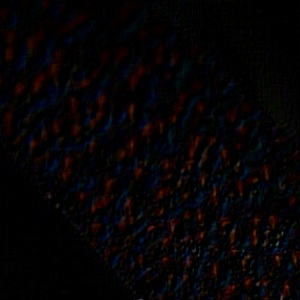
\includegraphics[width=0.2\textwidth]{resource/2-卷积.jpg}
    }
    \caption{卷积核的翻转对特征提取的影响}
    \label{Figure.Second.1}
  \end{figure}
  

  
  \subsection{\hei\xiaosan\textbf{卷积网络简介}}
    卷积网络(Convolutional Network),也叫卷积神经网络(Convolutional Neural Network,CNN),
    是一种具有局部连接、权重共享等特性的深层前馈神经网络,专门用来处理具有类似网格结构的数据的神经网络。
    

    1962年,Hubel和Wiesel通过对猫脑视觉皮层的研究,首次提出了一种新的概念——“感受野”
    (Receptive Field),对后来人工智能网络的发展起了很大的推动作用\cite{hubel1962receptive}。
    感受野是受生物学上感受野的机制而提出,在生物学上描述的是神经系统的一些神经元的特性。
    而在人工神经网络中,感受野指的是指的是卷积神经网络层输出的特征向量上的像素点对应的
    输入图像上的区域,通俗地讲,就是特征向量上的一个点对应的输入图像上的区域。1980年,Fukushima
    \cite{fukushima1982neocognitron}基于生物神经学的感受野理论提出了神经认知机和权重
    共享的卷积神经层,这被视为卷积神经网络的雏形。1989年,LeCun\cite{lecun1989backpropagation}
    将反向传播算法与权值共享的卷积神经层相结合,发明了卷积神经网络,并首次将卷积神经网络成功
    地应用到美国邮局的手写字符识别程序中。1998年,LeCun\cite{lecun1998gradient}提出了
    卷积神经网络的经典网络模型LeNet-5,它是第一个成功应用于数字\zs 识别问题的卷积神经网络。
    
 
  \subsection{\hei\xiaosan\textbf{卷积网络的特点}}
    % 卷积神经网络由神经认知机模型(Neocognitron)演变而来,由于其具有局部
    % 区域连接、权值共享、池化的结构特点,使得卷积神经网络在图像处理领域表现出色。与
    % 其他神经网络相比,卷积神经网络的特殊性表现在权值共享与局部连接等方面。权值共享使
    % 得卷积神经网络的网络结构与生物神经网络更加类似,从而更容易从中提取特征。局部连接
    % 不像传统神经网络那样,两个相连的网络层之间只有部分神经元互相连接,这两个特点很大
    % 程度上降低了网络模型的复杂度,减少了参数的数目,也提高了整个神经网络的训练效率。
    卷积运算通过三个重要的思想帮助改进深度学习系统:稀疏交互(Sparse Interactions)、
    参数\zs 共享(Parameter Sha\zs reing)和等变\zs 表示(Equivariant Represe\zs ntations)。
    
    稀疏交互的本质是对全连接的规避,这是通过使核的大小远小于输入的大小来达到的。当处理一
    张图像时,输入的图像可能包含几十万个像素点,但是我们可以使用只有数十个像素点的卷积核来
    达到提取特征的目的。这意味着我们不仅可以存储更少的参数,而且还大大减少了计算量,提高了
    统计效率。稀疏交互的图形化表示如图\ref{Figure.Second.2}所示。
    \begin{figure}[htbp]
      \centering
      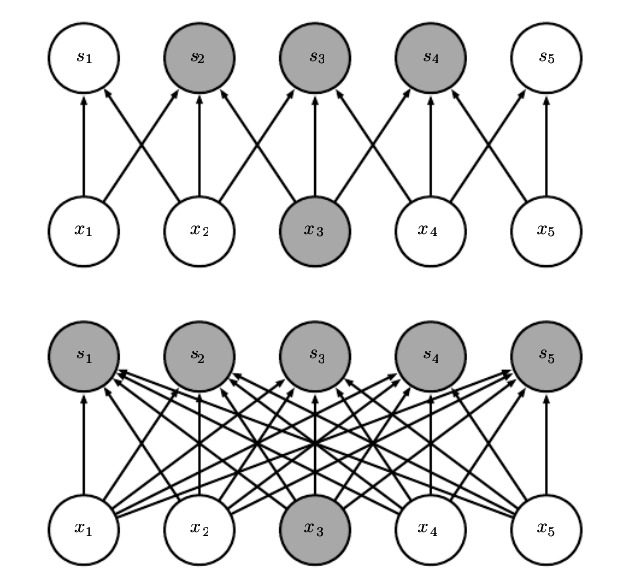
\includegraphics[width=.4\textwidth, natwidth=624, natheight=577]{resource/2.3-sparse.png}
      \caption{稀疏交互}
      \label{Figure.Second.2}
    \end{figure}
    
    参数共享是指在一个模型的多个函数中使用相同的参数。在传统的神经网络中,当计算一层的
    输出时,权重矩阵的每一个元素只使用一次,当它乘以输入的一个元素之后就再也用不到了。
    在卷积神经网络中,核的每一个元素都作用在输入的每一个位置上。参数\zs 共享保证了我们只需\zs 
    要学习一个参数\zs 集合,而不是每一个\zs 位置都需要学习一个新的\zs 集合。因此,卷积在存储需求和
    统计效率方面极大地优于稠密矩阵的乘法运算。

    在处理图像\zs 数据时,卷积产生\zs 了一个二维\zs 映射来表明某些特\zs 征在输入中出现的位\zs 置。
    如果我们移动输入中的图像,它的表示也会在输出中移动同样的量,这种性质就叫做等变表示。
    对于卷\zs 积来说,参数共\zs 享的特殊形式使\zs 得神经网络\zs 层具有对平移\zs 等变的性质。如果一个函数满足\zs 
    输入改变,输\zs 出也以同样的方式改\zs 变这一性质,我们\zs 就说它是等\zs 变的。特别的,如果函数$f(x)$与
    $g(x)$满\zs 足$f(g(x))=g(f(x))$,我们就说$f(x)$对于变换$g$具有等\zs 变性。对于卷积来说,
    如果令$g$是输\zs 入的任意平移函数,那么卷积\zs 函数对于$g$具有等变性。

  
  \subsection{\hei\xiaosan\textbf{卷积网络的结构}}
    卷积\zs 网络一般由数个卷\zs 积层(Convolu\zs tional layer)、池化层\zs (Pooling 
    layer)、全连\zs 接层及输出层交叉堆叠而成,卷积层和池化层一般会取多个,采用卷积层和
    池化层交替堆叠的模式。卷积层并\zs 行地计算多个卷积产生一组线性\zs 激活响应,每一个线性激活\zs 响应
    将会通过一个非线\zs 性的激活函数,例如整流\zs 线性激活函数。然后使用池\zs 化层来进一步调\zs 整这一层的输出。
    最后添加0~2个全连接层。
    目前,整个网络结构趋向于使用更小的卷积核(比如11和33)以及更深的网络结构。
    此外,由于卷积的操作性越来越灵活,池化层的作用也变得越来越小,因此目前比较流行的卷积网络中
    池化层的比例也越来越低,趋向于全卷积网络。
    
   


  \newpage
  \bibliographystyle{unsrt}
  \bibliography{references}

\end{document}
          